\documentclass[12pt]{beamer}
\usepackage{Estilos/BeamerFC}
\usepackage{Estilos/ColoresLatex}
\input{Preambulos/preambulo_Beamer_Warsaw_seahorse}
\usepackage{pifont}

\newcommand{\cmark}{\ding{51}}%
\newcommand{\xmark}{\ding{55}}%

\makeatletter
\setbeamertemplate{footline}
{
  \leavevmode%
  \hbox{%
  \begin{beamercolorbox}[wd=.333333\paperwidth,ht=2.25ex,dp=1ex,center]{section in foot}%
    \usebeamerfont{section in foot} \insertsection
  \end{beamercolorbox}%
  \begin{beamercolorbox}[wd=.333333\paperwidth,ht=2.25ex,dp=1ex,center]{subsection in foot}%
    \usebeamerfont{subsection in foot}  \insertsubsection
  \end{beamercolorbox}%
  \begin{beamercolorbox}[wd=.333333\paperwidth,ht=2.25ex,dp=1ex,right]{date in head/foot}%
    \usebeamerfont{date in head/foot} \insertshortdate{} \hspace*{2em}
    \insertframenumber{} / \inserttotalframenumber \hspace*{2ex} 
  \end{beamercolorbox}}%
  \vskip0pt%
}
\makeatother

\sisetup{
  per-mode=fraction,
  fraction-function=\tfrac
}

\setbeamertemplate{navigation symbols}{}
\date{1 de mayo}

% \sisetup{math-rm=\symup,detect-all}
\sisetup{detect-all, math-rm = \ensuremath}

\title{Sesión 11. Física}
\subtitle{Asesoría}

\begin{document}

\maketitle
\fontsize{14}{14}\selectfont
\spanishdecimal{.}

\section*{Contenido}
\frame[allowframebreaks]{\frametitle{Contenido} \tableofcontents[currentsection, hideallsubsections]}

\section{Segunda condición de equilibrio}
\frame{\frametitle{Temas a revisar} \tableofcontents[currentsection, hideothersubsections]}
\subsection{Definición}

\begin{frame}
\frametitle{Definición}
La \textocolor{blue}{segunda condición de equilibrio}, \pause también conocido como \textocolor{red}{condición de equilibrio rotacional}, \pause es una condición en la que un objeto o sistema en rotación se mantiene en reposo o en un movimiento de rotación constante y uniforme.
\end{frame}
% \begin{frame}
% \frametitle{La torca o momento angular}
% Se define a la \textocolor{red}{torca} de $\vb{F}$ con respecto a un punto de aplicación $O$ como el producto:
% \pause
% \begin{align*}
% \tau = F \cdot l
% \end{align*}
% Usaremos la letra griega $\tau$ (tau) para la torca.
% \end{frame}
% \begin{frame}
% \frametitle{Otros nombres para la torca}
% En física se prefiere el término \enquote{torca}, \pause mientras que los ingenieros prefieren el término \enquote{momento o par de torsión}
% \\
% \bigskip
% \pause
% A la distancia $l$ se la llama \enquote{brazo de palanca} o \enquote{brazo de momento}.
\begin{frame}
\frametitle{Segunda condición}
En otras palabras, \pause el objeto o sistema no experimenta una aceleración angular neta, \pause lo que significa que \textocolor{carmine}{la suma de todas las fuerzas y momentos} que actúan sobre el objeto o sistema \pause \textocolor{byzantine}{es igual a cero}.
\end{frame}
\begin{frame}
\frametitle{Segunda condición}
La segunda condición de equilibrio se puede expresar mediante la ley de Newton para la rotación, \pause que establece que la suma de los momentos de las fuerzas que actúan sobre un objeto debe ser igual a cero para que se mantenga en equilibrio rotacional.
\end{frame}
\begin{frame}
\frametitle{Segunda condición}
Es decir:
\pause
\begin{align*}
\nsum M = 0
\end{align*}
\pause
Donde $\nsum M$ es la suma de los momentos que actúan sobre el objeto.
\end{frame}
\begin{frame}
\frametitle{Expresión para el momento}
La expresión que nos determina el momento es:
\pause
\begin{align*}
M = F \cdot d
\end{align*}
\pause
donde:
\setbeamercolor{item projected}{bg=black,fg=white}
\setbeamertemplate{enumerate items}{%
\usebeamercolor[bg]{item projected}%
\raisebox{1.5pt}{\colorbox{bg}{\color{fg}\footnotesize\insertenumlabel}}%
}
\begin{enumerate}[<+->]
\item $M$ es el momento del objeto.
\item $F$ es la fuerza que actúa sobre un punto del objeto.
\item $d$ es la distancia medida del punto de apoyo al punto donde se aplica la fuerza.
\end{enumerate}
\end{frame}
\begin{frame}
\frametitle{Signo del momento}
\setbeamercolor{item projected}{bg=bananayellow,fg=blue}
\setbeamertemplate{enumerate items}{%
\usebeamercolor[bg]{item projected}%
\raisebox{1.5pt}{\colorbox{bg}{\color{fg}\footnotesize\insertenumlabel}}%
}
\begin{enumerate}[<+->]
\item El momento se considera \textocolor{cerise}{positivo} \pause si la fuerza tiende a hacer girar al cuerpo con respecto al eje de rotación en sentido opuesto al giro de las manecillas del reloj.
\\
\begin{figure}
  \centering
  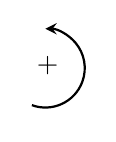
\begin{tikzpicture}
    \draw [-stealth, thick] (0, 0) arc(250:450:0.5);
    \node at (0.2, 0.5) {$+$};
  \end{tikzpicture}
\end{figure}
\seti
\end{enumerate}
\end{frame}
\begin{frame}
\frametitle{Signo del momento}
\setbeamercolor{item projected}{bg=bananayellow,fg=blue}
\setbeamertemplate{enumerate items}{%
\usebeamercolor[bg]{item projected}%
\raisebox{1.5pt}{\colorbox{bg}{\color{fg}\footnotesize\insertenumlabel}}%
}
\begin{enumerate}[<+->]
\conti
\item El momento se considera \textocolor{darkgreen}{negativo} \pause si la fuerza tiende a hacer girar al cuerpo con respecto al eje de rotación en el mismo sentido en que giran las mancillas del reloj.
\\
\begin{figure}
  \centering
  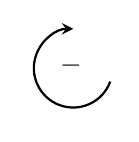
\begin{tikzpicture}
    \draw [-stealth, thick] (0, 0) arc(340:90:0.5);
    \node at (-0.5, 0.2) {$-$};
  \end{tikzpicture}
\end{figure}
\end{enumerate}
\end{frame}
\begin{frame}
\frametitle{Segunda condición}
El equilibrio rotacional es importante en la mecánica y la ingeniería, \pause ya que permite el diseño y la construcción de objetos y sistemas que deben mantenerse en rotación estable, como las ruedas de un automóvil, las aspas de un ventilador, las turbinas de una central hidroeléctrica, entre otros.
\end{frame}
\begin{frame}
\frametitle{Solución de problemas de equilibrio}
Consideremos que en la solución a problemas en donde se presenta la segunda condición de equilibrio, \pause tendremos que ocupar también la primera condición de equilibrio que ya hemos revisado.
\end{frame}

\subsection{Ejercicio 9 - Guía}

\begin{frame}
\frametitle{Enunciado del ejercicio}
Encontrar las reacciones $\vb{R}_{A}$ y $\vb{R}_{B}$ a las que se encuentra sujeto el apoyo en la siguiente viga.
\begin{figure}
  \centering
  \begin{tikzpicture}[scale=0.9]
    \draw [fill, color=bronze, draw=black] (0, 0) rectangle (9, 0.25);
    \draw [fill, color=brightturquoise, draw=black] (0, 0) -- (0.5, -0.5) -- (-0.5, -0.5) node [below, midway, text=black] {\small{$\vb{R}_{A}$}} -- cycle;
    \draw [fill, color=brightturquoise, draw=black] (9, 0) -- (9.5, -0.5) -- (8.5, -0.5) node [below, midway, text=black] {\small{$\vb{R}_{B}$}} -- cycle;
    \draw [-stealth, thick] (0, 1.5) -- (0, 0.25);
    \node at (0, 1.8) {\small{$F_{1} = \SI{70}{\newton}$}};
    
    \draw [-stealth, thick] (2, 1.5) -- (2, 0.25);
    \node at (2, 1.8) {\small{$F_{2} = \SI{68}{\newton}$}};
    \draw [-stealth, <->] (0, 1.3) -- (2, 1.3) node [below, midway] {\small{$\SI{2}{\meter}$}};

    \draw [-stealth, thick] (5.5, 1.5) -- (5.5, 0.25);
    \node at (5.5, 1.8) {\small{$F_{3} = \SI{92}{\newton}$}};
   
    \draw [-stealth, thick] (9, 1.5) -- (9, 0.25);
    \node at (9, 1.8) {\small{$F_{4} = \SI{68}{\newton}$}};
   
    \draw [-stealth, <->] (5.5, 1.3) -- (9, 1.3) node [below, midway] {\small{$\SI{4}{\meter}$}};

    \draw [-stealth, thick] (9, 0.12) -- (10, 0.12) node [above, pos=1.1] {\small{$F_{5} = \SI{25}{\newton}$}};

    % \onslide<1->
  \end{tikzpicture}
\end{figure}
\end{frame}
\begin{frame}
\frametitle{Enunciado del Ejercicio 9}
La masa de la viga es de \SI{65}{\kilo\gram} y tiene una longitud de \SI{12}{\meter}.
\end{frame}
\begin{frame}
\frametitle{Pasos para resolver}
\textocolor{black}{1. Elaborar el diagrama de cuerpo libre del sistema.}
\\
\bigskip
\pause
Recordemos que para ello, es necesario tomar en cuenta todas las fuerzas que actúan en este caso, sobre la barra, \pause incluido su peso.
\end{frame}
\begin{frame}
\frametitle{Peso de la barra}
El peso de la barra $W$, \pause lo obtenemos al multiplicar el valor de la masa $m = \SI{65}{\kilo\gram}$ por el valor de $g = \SI{9.81}{\meter\per\square\second}$:
\pause
\begin{eqnarray*}
\begin{aligned}
W &= m \cdot g = (\SI{65}{\kilo\gram})(\SI{9.81}{\meter\per\square\second}) = \\[0.5em] \pause
&= \SI{637.65}{\kilo\gram\meter\per\square\second} = \\[0.5em] \pause
&= \SI{637.65}{\newton}
\end{aligned}
\end{eqnarray*}
\end{frame}
\begin{frame}
\frametitle{El peso de la viga}
Ya hemos calculado el peso de la viga, \pause pero falta determinar el punto en donde este vector $W$ actúa sobre la misma viga.
\\
\bigskip
\pause
El punto de aplicación corresponde al punto medio de la viga, es decir, \SI{6}{\meter}.
\end{frame}
\begin{frame}
\frametitle{Diagrama de cuerpo libre}
Representaremos las reacciones $\vb{R}_{A}$ y $\vb{R}_{B}$ como vectores, así como el peso $W$:
\pause
\begin{figure}
  \centering
  \begin{tikzpicture}[scale=0.9]
    \draw [fill, color=bronze, draw=black] (0, 0) rectangle (9, 0.25);
    % \draw [fill, color=brightturquoise, draw=black] (0, 0) -- (0.5, -0.5) -- (-0.5, -0.5) node [below, midway, text=black] {\small{$\vb{R}_{A}$}} -- cycle;
    % \draw [fill, color=brightturquoise, draw=black] (9, 0) -- (9.5, -0.5) -- (8.5, -0.5) node [below, midway, text=black] {\small{$\vb{R}_{B}$}} -- cycle;

    \draw [-stealth, thick] (0, -1.5) -- (0, 0) node [right, midway] {\small{$R_{A}$}};
    \draw [-stealth, thick] (9, -1.5) -- (9, 0) node [left, midway] {\small{$R_{B}$}};

    \draw [-stealth, thick] (0, 1.5) -- (0, 0.25);
    \node at (0, 1.8) {\small{$F_{1}$}};
    
    \draw [-stealth, thick] (2, 1.5) -- (2, 0.25);
    \node at (2, 1.8) {\small{$F_{2}$}};
    \draw [-stealth, <->] (0, 1.3) -- (2, 1.3) node [below, midway] {\small{$\SI{2}{\meter}$}};

    \draw [-stealth, thick] (4.5, 0) -- (4.5, -2) node [right, midway] {\small{$W$}};
    \draw (0, -2) -- (0, -2.4);
    \draw (4.5, -2) -- (4.5, -2.4);
    \draw [-stealth, <->](0, -2.2) -- (4.5, -2.2) node [above, midway] {\small{$\SI{6}{\meter}$}};

    \draw [-stealth, thick] (5.5, 1.5) -- (5.5, 0.25);
    \node at (5.5, 1.8) {\small{$F_{3}$}};
   
    \draw [-stealth, thick] (9, 1.5) -- (9, 0.25);
    \node at (9, 1.8) {\small{$F_{4}$}};
   
    \draw [-stealth, <->] (5.5, 1.3) -- (9, 1.3) node [below, midway] {\small{$\SI{4}{\meter}$}};

    \draw [-stealth, thick] (9, 0.12) -- (10, 0.12) node [above, pos=1.1] {\small{$F_{5}$}};

    % \onslide<1->
  \end{tikzpicture}
\end{figure}
\end{frame}
\begin{frame}
\frametitle{Siguiente paso}
\textocolor{black}{2. Calculando los momentos.}
\\
\bigskip
\pause
Tomemos en cuenta que para cada una de las fuerzas $\vb{F}_{i}$ que aparecen en el DCL, tendremos asociado un momento, de tal manera que es en esta parte donde aplicamos la segunda condición de equilibrio.
\pause
\begin{align*}
\nsum_{i} M_{i} = 0
\end{align*}
\end{frame}
\begin{frame}
\frametitle{Regla recomendada}
Comenzamos de \textocolor{carmine}{izquierda a derecha}, siendo el punto de aplicación $O$, donde tenemos el soporte izquierdo de la viga:
\pause
\begin{eqnarray*}
\begin{aligned}
\nsum M = d_{1} \, R_{A} {-} d_{1} \, F_{1} {-} d_{2} \, F_{2} {-} d_{3} \, F_{3} {-} d_{4} \, F_{4} {+} d_{4} \, R_{B} {=} 0
\end{aligned}
\end{eqnarray*}
\end{frame}
\begin{frame}
\frametitle{Sobre los signos}
\begin{eqnarray*}
\begin{aligned}
\nsum M = d_{1} \, R_{A} {-} d_{1} \, F_{1} {-} d_{2} \, F_{2} {-} d_{3} \, F_{3} {-} d_{4} \, F_{4} {+} d_{4} \, R_{B} {=} 0
\end{aligned}
\end{eqnarray*}
\pause
Los signos $(-)$ corresponden a los momentos que están en el sentido de las manecillas del reloj, mientras que los signos $(+)$ son para los momentos en sentido contrario a las manecillas del reloj.
\end{frame}
\begin{frame}
\frametitle{De la fuerza $F_{5}$}
La fuerza $F_{5}$ no se incluye en la expresión anterior, \pause ya que es paralela al eje de rotación de la viga.
\\
\bigskip
\pause
Recordemos que se presenta un momento, siempre y cuando la fuerza sea perpendicular al eje de rotación.
\end{frame}
\begin{frame}
\frametitle{Tomando las distancias}
Para hacer las cuentas, necesitamos obtener las distancias, por lo que:
\begin{eqnarray*}
\begin{aligned}
d_{1} &= 0 \hspace{1.5cm} \pause d_{2} = \SI{2}{\meter} \\[0.5em] \pause
d_{3} &= \SI{8}{\meter} \hspace{1.5cm} \pause d_{4} = \SI{12}{\meter}
\end{aligned}
\end{eqnarray*}
\end{frame}
\begin{frame}
\frametitle{Haciendo las cuentas}
Tenemos que:
\pause
\begin{eqnarray*}
\begin{aligned}
&\nsum M = \Cancel[red]{d_{1} \, R_{A}} {-} \Cancel[red]{d_{1} \, F_{1}} {-} d_{2} \, F_{2} {-} d_{3} \, F_{3} {-} d_{4} \, F_{4} {+} d_{4} \, R_{B} {=} 0 \\[0.5em] \pause
&- (\SI{2}{\meter})(\SI{68}{\newton}) {-} (\SI{8}{\meter})(\SI{92}{\newton}) {-} (\SI{12}{\meter})(\SI{68}{\newton}) {+}  \\[0.5em]
&+ (\SI{12}{\meter})(R_{B}) = 0 \\[0.5em] \pause
& - \SI{136}{\meter\newton} - \SI{736}{\meter\newton} - \SI{816}{\meter\newton} + (\SI{12}{\meter})(R_{B}) = 0 \\[0.5em] \pause
& - \SI{1688}{\meter\newton} + (\SI{12}{\meter})(R_{B}) = 0
\end{aligned}
\end{eqnarray*}
\end{frame}
\begin{frame}
\frametitle{Haciendo las cuentas}
\begin{eqnarray*}
\begin{aligned}
(\SI{12}{\meter})(R_{B}) &= - \SI{1688}{\meter\newton} \\[0.5em] \pause
R_{B} &= \dfrac{\SI{1688}{\meter\newton}}{\SI{12}{\meter}} \\[0.5em] \pause
R_{B} &= \SI{140.66}{\newton}
\end{aligned}
\end{eqnarray*}
\end{frame}
\begin{frame}
\frametitle{Siguiente paso}
\textocolor{black}{3. Usar la primera condición de equilibrio.}
\\
\bigskip
\pause
Para recuperar la reacción $\vb{R}_{A}$, aplicamos la primera condición de equilibrio:
\pause
\begin{align*}
\nsum_{i} F_{i} = 0
\end{align*}
donde las $F_{i}$ son todas las fuerzas que actúan sobre la viga.
\end{frame}
\begin{frame}
\frametitle{Primera condición de equilibrio}
Se tiene entonces que:
\pause
\begin{eqnarray*}
\begin{aligned}
&\nsum_{i} F_{i} = 0 \\[0.5em] \pause
&= R_{A} - F_{1} - F_{2} - F_{3} - F_{4} + R_{B} = 0
\end{aligned}
\end{eqnarray*}
Los signos corresponden a la dirección que tiene cada una de las fuerzas involucradas.
\end{frame}
\begin{frame}
\frametitle{Haciendo las cuentas}
Resolvemos la primera condición de equilibrio:
\pause
\begin{eqnarray*}
\begin{aligned}
&\nsum_{i} F_{i} = R_{A} - F_{1} - F_{2} - F_{3} - F_{4} + R_{B} = 0 \\[0.5em] \pause
& R_{A} = F_{1} + F_{2} + F_{3} + F_{4} - R_{B} = 0
\end{aligned}
\end{eqnarray*}  
\end{frame}
\begin{frame}
\frametitle{Sustituyendo los valores}
Al ocupar los valores de las $F_{i}$ y de $R_{B}$:
\pause
\begin{eqnarray*}
\begin{aligned}
R_{A} &= F_{1} + F_{2} + F_{3} + F_{4} - R_{B} = \\[0.5em] \pause
& = \SI{70}{\newton} + \SI{68}{\newton} + \SI{92}{\newton} + \SI{68}{\newton} - \SI{140.66}{\newton} = \\[0.5em] \pause
R_{A} &= \SI{157.34}{\newton}
\end{aligned}
\end{eqnarray*}
\end{frame}
\begin{frame}
\frametitle{Solución al Ejercicio 9}
Hemos obtenido el valor de las reacciones debajo de la viga:
\begin{align*}
R_{A} &= \SI{157.34}{\newton} \\[0.5em]
R_{B} &= \SI{140.66}{\newton}
\end{align*}
\end{frame}

\subsection{Ejercicio 10 - Guía}

\begin{frame}
\frametitle{Enunciado del Ejercicio 10}
Encontrar las reacciones $\vb{R}_{A}$ y $\vb{R}_{B}$ a las que se encuentra sujeto el apoyo en la siguiente viga.
\begin{figure}
  \centering
  \begin{tikzpicture}[scale=0.9]
    \draw [fill, color=bronze, draw=black] (0, 0) rectangle (9, 0.25);
    \draw [fill, color=brightturquoise, draw=black] (0, 0) -- (0.5, -0.5) -- (-0.5, -0.5) node [below, midway, text=black] {\small{$\vb{R}_{A}$}} -- cycle;
    \draw [fill, color=brightturquoise, draw=black] (7, 0) -- (7.5, -0.5) -- (6.5, -0.5) node [below, midway, text=black] {\small{$\vb{R}_{B}$}} -- cycle;
    \draw [-stealth, thick] (0, 1.5) -- (0, 0.25);
    \node at (0, 1.8) {\small{$F_{1} = \SI{10}{\newton}$}};
    
    \draw [-stealth, thick] (3, 1.5) -- (3, 0.25);
    \node at (3, 1.8) {\small{$F_{2} = \SI{13}{\newton}$}};
    \draw [-stealth, <->] (0, 1.3) -- (3, 1.3) node [below, midway] {\small{$\SI{5}{\meter}$}};

    \draw [-stealth, thick] (7, 1.5) -- (7, 0.25);
    \node at (7, 1.8) {\small{$F_{3} = \SI{44}{\newton}$}};
    
    \draw [-stealth, thick] (9, 1.5) -- (9, 0.25);
    \node at (9, 1.8) {\small{$F_{4} = \SI{22}{\newton}$}};
    
    \draw [-stealth, <->] (7, 1.3) -- (9, 1.3) node [below, midway] {\small{$\SI{3}{\meter}$}};
    
    % \onslide<1->
  \end{tikzpicture}
\end{figure}
\end{frame}
\begin{frame}
\frametitle{Enunciado del Ejercicio 10}
El peso de la viga es de \SI{70}{\newton} y tiene una longitud de \SI{20}{\meter}.
\\
\bigskip
\pause
Notemos que el punto de apoyo del lado derecho, no se encuentra en el extremo derecho de la viga.
\end{frame}
\begin{frame}
\frametitle{Siguiendo los pasos}
Nuevamente repetimos los pasos para resolver el ejercicio, de esta manera tendremos de manera organizada el procedimiento.
\end{frame}
\begin{frame}
\frametitle{Paso 1. Elaborando el DCL}
El enunciado ya nos indica el peso $W$ de la viga, por lo que nuestro DCL queda como:
\pause
\begin{figure}
  \centering
  \begin{tikzpicture}[scale=0.9]
    \draw [fill, color=bronze, draw=black] (0, 0) rectangle (9, 0.25);
    \draw [-stealth, thick] (0, -1.5) -- (0, 0) node [left, midway] {\small{$\vb{R}_{A}$}};
    \draw [-stealth, thick] (7, -1.5) -- (7, 0) node [right, midway] {\small{$\vb{R}_{B}$}};

    \draw [-stealth, thick] (0, 1.5) -- (0, 0.25);
    \node at (0, 1.8) {\small{$F_{1}$}};
    
    \draw [-stealth, thick] (2, 1.5) -- (2, 0.25);
    \node at (2, 1.8) {\small{$F_{2}$}};
    \draw [-stealth, <->] (0, 1.3) -- (2, 1.3) node [below, midway] {\small{$\SI{5}{\meter}$}};

    \draw [-stealth, thick] (4.5, 0) -- (4.5, -2) node [left, midway] {\small{$W$}};
    \draw (0, -2) -- (0, -2.4);
    \draw (4.5, -2) -- (4.5, -2.4);
    \draw [-stealth, <->](0, -2.2) -- (4.5, -2.2) node [above, midway] {\small{$\SI{10}{\meter}$}};

    \draw [-stealth, thick] (7, 1.5) -- (7, 0.25);
    \node at (7, 1.8) {\small{$F_{3}$}};
    
    \draw [-stealth, thick] (9, 1.5) -- (9, 0.25);
    \node at (9, 1.8) {\small{$F_{4}$}};
    
    \draw [-stealth, <->] (7, 1.3) -- (9, 1.3) node [below, midway] {\small{$\SI{3}{\meter}$}};
    
    % \onslide<1->
  \end{tikzpicture}
\end{figure}
\end{frame}
\begin{frame}
\frametitle{Siguiente paso}
\textocolor{black}{2. Calculando los momentos.}
Expresamos la segunda condición de equilibrio:
\pause
\begin{align*}
\nsum_{i} M_{i} = 0
\end{align*}
Ocupando las fuerzas que se indican en el DCL.
\end{frame}
\begin{frame}
\frametitle{Segunda condición de equilibrio}
Por lo que:
\pause
\begin{eqnarray*}
\begin{aligned}
&\nsum_{i} M_{i} = 0 \\[0.5em] \pause
&-d_{1} F_{1} + d_{1} R_{A} - d_{2} F_{2} - d_{3} F_{3} + d_{3} R_{B} - d_{4} F_{4} = 0 \\[0.5em] \pause
&- d_{2} F_{2} - d_{3} F_{3} + d_{3} R_{B} - d_{4} F_{4} = 0 \\[0.5em] \pause
&- (\SI{5}{\meter})(\SI{13}{\newton}) - (\SI{17}{\meter})(\SI{44}{\newton}) + \\[0.5em]
&+ (\SI{17}{\meter})(R_{B}) - (\SI{20}{\meter})(\SI{22}{\newton}) = 0
\end{aligned}
\end{eqnarray*}
\end{frame}
\begin{frame}
\frametitle{Segunda condición de equilibrio}
\begin{eqnarray*}
\begin{aligned}
&- (\SI{5}{\meter})(\SI{13}{\newton}) - (\SI{17}{\meter})(\SI{44}{\newton}) + \\[0.5em]
&+ (\SI{17}{\meter})(R_{B}) - (\SI{20}{\meter})(\SI{22}{\newton}) = 0 \\[0.5em] \pause
& - \SI{65}{\meter\newton} - \SI{748}{\meter\newton} + (\SI{17}{\meter})(R_{B}) - \SI{440}{\meter\newton} = 0 \\[0.5em] \pause
& - \SI{1253}{\meter\newton} + (\SI{17}{\meter})(R_{B}) = 0
\end{aligned}
\end{eqnarray*}
\end{frame}
\begin{frame}
\frametitle{Obteniendo $R_{B}$}
Despejamos el valor de $R_{B}$:
\pause
\begin{eqnarray*}
\begin{aligned}
- \SI{1253}{\meter\newton} + (\SI{17}{\meter})(R_{B}) &= 0 \\[0.5em] \pause
(\SI{17}{\meter})(R_{B}) &= \SI{1253}{\meter\newton} \\[0.5em] \pause
R_{B} &= \dfrac{\SI{1253}{\meter\newton}}{\SI{17}{\meter}} \\[0.5em] \pause
R_{B} &= \SI{73.70}{\newton}
\end{aligned}
\end{eqnarray*}
\end{frame}
\begin{frame}
\frametitle{Siguiente paso}
\textocolor{black}{3. Usar la primera condición de equilibrio.}
\\
\bigskip
\pause
Para recuperar la reacción $\vb{R}_{A}$, aplicamos la primera condición de equilibrio:
\pause
\begin{align*}
\nsum_{i} F_{i} = 0
\end{align*}
donde las $F_{i}$ son todas las fuerzas que actúan sobre la viga.
\end{frame}
\begin{frame}
\frametitle{Primera condición de equilibrio}
Se tiene entonces que:
\pause
\begin{eqnarray*}
\begin{aligned}
&\nsum_{i} F_{i} = 0 \\[0.5em] \pause
&= R_{A} - F_{1} - F_{2} - F_{3} + R_{B} - F_{4} = 0
\end{aligned}
\end{eqnarray*}
Los signos corresponden a la dirección que tiene cada una de las fuerzas involucradas.
\end{frame}
\begin{frame}
\frametitle{Haciendo las cuentas}
Sustituimos los valores de las fuerzas, para luego despejar $R_{A}$:
\pause
\begin{eqnarray*}
\begin{aligned}
&R_{A} - F_{1} - F_{2} - F_{3} + R_{B} - F_{4} = 0 \\[0.5em] \pause
&R_{A} = F_{1} + F_{2} + F_{3} - R_{B} + F_{4} \\[0.5em] \pause
&R_{A} = \SI{10}{\newton} + \SI{13}{\newton} + \SI{44}{\newton} - \SI{73.70}{\newton} + \SI{220}{\newton} \\[0.5em] \pause
&R_{A} = \SI{213.30}{\newton}
\end{aligned}
\end{eqnarray*}
\end{frame}
\begin{frame}
\frametitle{Solución al Ejercicio 10}
Hemos obtenido el valor de las reacciones debajo de la viga:
\begin{align*}
R_{A} &= \SI{213.30}{\newton} \\[0.5em]
R_{B} &= \SI{73.70}{\newton}
\end{align*}
\end{frame}

\subsection{Ejercico 11 - Guía}

\begin{frame}
\frametitle{Enunciado del Ejercicio 11}
Encontrar las reacciones $\vb{R}_{A}$ y $\vb{R}_{B}$ a las que se encuentra sujeto el apoyo en la siguiente viga:
\begin{figure}
  \centering
  \begin{tikzpicture}[scale=0.9]
    \draw [fill, color=bronze, draw=black] (0, 0) rectangle (9, 0.25);
    \draw [fill, color=brightturquoise, draw=black] (2, 0) -- (2.5, -0.5) -- (1.5, -0.5) node [below, midway, text=black] {\small{$\vb{R}_{A}$}} -- cycle;
    \draw [fill, color=brightturquoise, draw=black] (7, 0) -- (7.5, -0.5) -- (6.5, -0.5) node [below, midway, text=black] {\small{$\vb{R}_{B}$}} -- cycle;

    \draw [-stealth, thick] (0, 1.5) -- (0, 0.25);
    \node at (0, 1.8) {\small{$F_{1} = \SI{7}{\newton}$}};

    \draw [dashed] (2, 0.25) -- (2, 1.7);
    \draw [-stealth, <->] (0, 1.3) -- (2, 1.3) node [below, midway] {\small{$\SI{5}{\meter}$}};
    \draw [dashed] (3, 0.25) -- (3, 1.7);
    \draw [-stealth, <->] (2, 1.3) -- (3, 1.3) node [below, midway] {\small{$\SI{2}{\meter}$}};

    \draw [-stealth, thick] (3, 0.25) -- (4.73, 1);
    \node at (4.5, 1.8) {\small{$F_{2} = \SI{16}{\newton}$}};
    \draw (3.5, 0.25) arc(0:30:0.4);
    \node at (4.5, 0.5) {\footnotesize{$\theta = \ang{30}$}};

    \draw [-stealth, thick] (7, 1.5) -- (7, 0.25);
    \node at (7, 1.8) {\small{$F_{3} = \SI{26}{\newton}$}};
    
    \draw [-stealth, thick] (9, 1.5) -- (9, 0.25);
    \node at (9, 1.8) {\small{$F_{4} = \SI{10}{\newton}$}};
    
    \draw [-stealth, <->] (7, 1.3) -- (9, 1.3) node [below, midway] {\small{$\SI{4}{\meter}$}};
    
    % \onslide<1->
  \end{tikzpicture}
\end{figure}
\end{frame}

\end{document}